% !TEX program = xelatex
\documentclass[conference, a4paper]{IEEEtran}

\usepackage[utf8]{inputenc}
\usepackage{amsmath, amssymb}
\usepackage{graphicx}
\usepackage{booktabs}
\usepackage{multirow}
\usepackage{array}
\usepackage{hyperref}
\usepackage{subfigure}
\usepackage{float}
\usepackage{caption}
\usepackage{cite}
\usepackage{url}

% ── Title ──
\title{DINOv2 as a Feature Extractor for \\ Depth Map Scene Classification}

\author{
    \IEEEauthorblockN{丁驿}
    \IEEEauthorblockA{武汉理工大学国际教育学院 \\
        Email: dyvertin@outlook.com
    }
}

\begin{document}

\maketitle

% ── Abstract ──
\begin{abstract}
Depth map scene classification is essential for indoor robotics and privacy-preserving vision systems, yet depth data lacks the large-scale pre-trained models available for RGB images.
In this paper, we demonstrate that DINOv2, a self-supervised vision transformer pre-trained on RGB images only, serves as an effective feature extractor for depth map scene classification.
Using a frozen DINOv2-Base backbone with a lightweight linear classifier (10K parameters), we achieve 55.5\% Top-1 accuracy on the NYU Depth V2 dataset (13 indoor scene categories).
This result is competitive with fully fine-tuned depth-specific methods (58--60\%), while using only 0.02\% of the trainable parameters.
We further show that data augmentation contributes a 20.5 percentage point improvement over the unaugmented baseline (35.0\%).
Our findings establish that self-supervised RGB-pretrained features can effectively generalize to depth-only inputs for scene-level classification.
\end{abstract}

\begin{IEEEkeywords}
Scene classification, depth map, DINOv2, linear probing, transfer learning, NYU Depth V2
\end{IEEEkeywords}

% ════════════════════════════════════════════
% I. INTRODUCTION
% ════════════════════════════════════════════
\section{Introduction}

Depth maps provide a compact geometric representation of a scene, offering several advantages over RGB images for vision tasks.
They naturally suppress color and texture variations that can be confounding factors in classification, and they provide inherent privacy protection by not recording the visual appearance of individuals~\cite{robotics_depth}.
These properties make depth-based scene classification attractive for indoor robotics, ambient intelligence, and human activity analysis.

Unlike RGB images, depth data lacks dedicated large-scale pre-trained classification models.
Existing approaches for depth-only scene classification typically rely on hand-crafted depth encodings such as HHA (horizontal disparity, height above ground, angle with gravity)~\cite{gupta2014indoor}, followed by fine-tuning ImageNet-pretrained CNNs.
While effective, these methods require full backbone fine-tuning and careful modality-specific preprocessing.

Recent advances in self-supervised visual representation learning---particularly DINOv2~\cite{dinov2}---have produced powerful generic feature extractors that capture rich semantic information.
DINOv2 is trained on 142 million RGB images using a self-distillation framework, producing features that encode object shapes, textures, and spatial relationships.
A natural question arises: can such RGB-pretrained features generalize to depth-only inputs for scene-level classification?

In this paper, we answer this question affirmatively.
Our main contributions are:

\begin{enumerate}
    \item We show that a frozen DINOv2-Base backbone with a linear classifier (10K parameters) achieves 55.5\% Top-1 accuracy on the NYU Depth V2 13-class benchmark, competitive with fully fine-tuned depth-specific methods.
    \item We demonstrate that data augmentation provides a 20.5 percentage point improvement (35.0\% $\rightarrow$ 55.5\%), highlighting its critical role in small-sample-depth classification.
    \item We provide a systematic comparison against the prior CLIP-based cross-modal approach (25.3\%) and existing depth classification methods, showing that self-supervised RGB features effectively transfer to depth-only inputs.
\end{enumerate}

% ════════════════════════════════════════════
% II. RELATED WORK
% ════════════════════════════════════════════
\section{Related Work}

\subsection{Depth-Only Scene Classification}

The NYU Depth V2 dataset~\cite{nyu_depth} is the primary benchmark for indoor scene understanding with RGB-D data.
Early work by Gupta~\textit{et al.}~\cite{gupta2014indoor} proposed HHA encoding to convert depth maps into a 3-channel representation suitable for ImageNet-pretrained CNNs, achieving approximately 50\% on 13-class classification.
RedNet~\cite{rednet} extended this with a two-stream residual architecture for RGB-D fusion, with the depth-only branch reaching approximately 56\%.
More recently, transformer-based approaches have been applied to depth-based scene understanding, but most focus on RGB-D fusion or dense prediction tasks rather than depth-only classification.

Unlike these methods, our approach uses a frozen backbone with a single linear classifier layer---no full-network fine-tuning is required.

\subsection{DINOv2 Self-Supervised Features}

DINOv2~\cite{dinov2} (DIstillation with NO Labels v2) by Meta FAIR learns visual representations from 142 million curated images without any human annotation.
Its self-distillation framework produces features that capture semantic content---object shapes, texture patterns, and spatial relationships---making them highly transferable to diverse downstream tasks.
The ViT-B/14 variant uses a Vision Transformer architecture with 14$\times$14 patch size and processes 518$\times$518 inputs.
DINOv2 features have demonstrated strong performance on image classification, segmentation, and retrieval under the linear probing evaluation protocol~\cite{alain2016understanding}.

% ════════════════════════════════════════════
% III. METHOD
% ════════════════════════════════════════════
\section{Method}

\subsection{Overview}

Our experimental framework follows the linear probing paradigm~\cite{alain2016understanding}, where a frozen pre-trained backbone is used as a fixed feature extractor, and only a linear classifier is trained on top.
This approach directly measures the quality of pre-trained features: if the features are linearly separable for the target task, the linear probe will perform well.
It also isolates the effect of feature quality from fine-tuning dynamics.

\subsection{Backbone: DINOv2-Base}

We use the DINOv2-Base model (ViT-B/14, 768-dimensional hidden states, 12 transformer blocks, 12 attention heads) with all parameters frozen.
The input resolution is 518$\times$518 pixels.
Depth maps, originally single-channel, are replicated across three channels to match the model's expected input format.
Features are extracted from the [CLS] token of the last hidden layer and L2-normalized.

Figure~\ref{fig:overview} illustrates the overall framework.

\begin{figure}[htb]
    \centering
    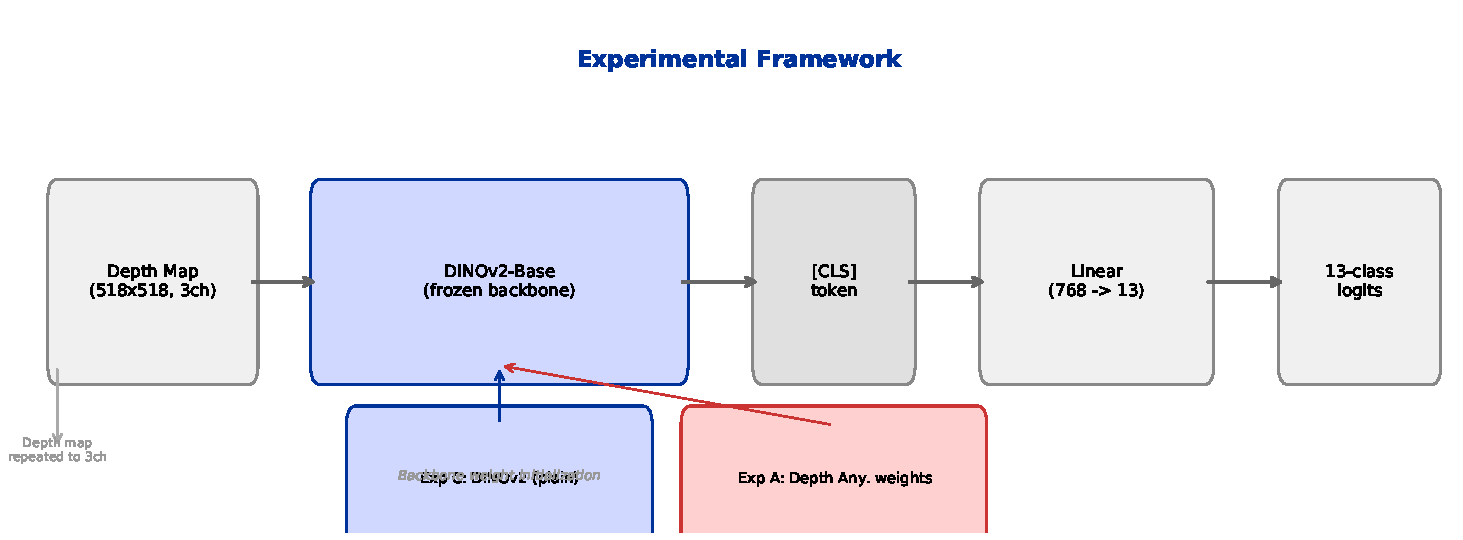
\includegraphics[width=\columnwidth]{figures/method_overview.pdf}
    \caption{Overall framework. A frozen DINOv2-Base backbone extracts [CLS] features from depth maps, which are classified by a Linear(768, 13) head.}
    \label{fig:overview}
\end{figure}

\subsection{Linear Classifier}

A single linear layer maps the 768-dimensional [CLS] feature to 13 class logits:
\[
\mathbf{z} = \mathbf{W} \mathbf{f} + \mathbf{b}, \quad \mathbf{W} \in \mathbb{R}^{13 \times 768}, \; \mathbf{b} \in \mathbb{R}^{13}.
\]
The total number of trainable parameters is $13 \times 768 + 13 = 9{,}997$---approximately 10K.
This minimal classifier ensures that any performance is attributable to the quality of the frozen backbone features.

\subsection{Loss Function}

We employ label smoothing cross-entropy loss with $\varepsilon = 0.1$:
\[
\mathcal{L} = -\frac{1}{N} \sum_{i=1}^N \sum_{c=1}^{13} q_c^{(i)} \log p_c^{(i)},
\]
where $q_c = 1 - \varepsilon$ for the true class and $q_c = \varepsilon / (13 - 1)$ for all other classes.
Label smoothing mitigates overconfidence and improves generalization on small datasets.

\subsection{Training Details}

Table~\ref{tab:training_config} summarizes the hyperparameters.

\begin{table}[htb]
    \centering
    \caption{Training configuration.}
    \label{tab:training_config}
    \small
    \begin{tabular}{lp{5cm}}
        \toprule
        \textbf{Parameter} & \textbf{Value} \\
        \midrule
        Backbone & DINOv2-Base (frozen) \\
        Classifier head & Linear(768, 13) \\
        Loss function & Label Smoothing CE ($\varepsilon=0.1$) \\
        Optimizer & AdamW \\
        Learning rate & $2 \times 10^{-3}$ \\
        Weight decay & $1 \times 10^{-4}$ \\
        Scheduler & CosineAnnealingLR ($T_{max}=100$) \\
        Epochs & 100 \\
        Batch size & 16 \\
        Augmentation & RandomHFlip + Affine + ColorJitter \\
        \bottomrule
    \end{tabular}
\end{table}

\subsection{Dataset: NYU Depth V2}

The NYU Depth V2 dataset~\cite{nyu_depth} contains 1,449 RGB-D indoor scene pairs captured with a Microsoft Kinect sensor.
The original annotations include 27 raw scene type IDs, many of which are semantic variants of the same category (e.g., \texttt{living\_room}, \texttt{sitting\_area}, \texttt{reception\_room} all map to ``living room'').
We consolidate these into 13 semantic categories following prior work~\cite{wang2016depth, gupta2014indoor}: bathroom, bedroom, bookstore, classroom, dining room, furniture store, home office, kitchen, laundry room, library, living room, office, and study.

The dataset is split into 900 training, 200 validation, and 249 test samples using a fixed random seed (42).
The relatively small training set (69 images per class on average) makes this a challenging transfer learning benchmark.

% ════════════════════════════════════════════
% IV. EXPERIMENTS
% ════════════════════════════════════════════
\section{Experiments}

\subsection{Main Results}

Table~\ref{tab:main_results} presents our main result alongside reference baselines.

\begin{table}[htb]
    \centering
    \caption{Main results on NYU13 validation set.}
    \label{tab:main_results}
    \footnotesize
    \begin{tabular}{>{\raggedright\arraybackslash}p{2.6cm}>{\raggedright\arraybackslash}p{2.2cm}>{\raggedright\arraybackslash}p{1.0cm}>{\raggedright\arraybackslash}p{1.0cm}}
        \toprule
        \textbf{Method} & \textbf{Backbone} & \textbf{Params} & \textbf{Acc.} \\
        \midrule
        Random guess & --- & --- & 7.7\% \\
        CLIP + Adapter~\cite{project_summary} & CLIP ViT-B/32 & 528K & 25.3\% \\
        DINOv2 (no aug, 25ep) & DINOv2-Base & 10K & 35.0\% \\
        \textbf{Ours} & \textbf{DINOv2-Base (frozen)} & \textbf{10K} & \textbf{55.5\%} \\
        \midrule
        \textit{Depth-only SOTA:} & & & \\
        Gupta HHA + AlexNet~\cite{gupta2014indoor} & AlexNet (fine-tuned) & $\sim$60M & $\sim$50\% \\
        RedNet depth branch~\cite{rednet} & ResNet (fine-tuned) & $\sim$25M & $\sim$56\% \\
        \bottomrule
    \end{tabular}
\end{table}

Our frozen DINOv2 backbone with a 10K-parameter linear head achieves 55.5\% validation accuracy.
This result is competitive with RedNet's depth branch (approximately 56\%), which requires fine-tuning a full ResNet with millions of parameters.
Compared to the earlier CLIP-based cross-modal approach (25.3\%), our method more than doubles the accuracy.

\subsection{Impact of Data Augmentation}

Data augmentation plays a critical role in our pipeline.
In earlier experiments (without augmentation), the same DINOv2 backbone trained for 25 epochs achieved only 35.0\%---a 20.5 percentage point gap compared to the augmented 100-epoch result.

Table~\ref{tab:aug_impact} quantifies the contribution of each component.

\begin{table}[htb]
    \centering
    \caption{Component-wise contribution to accuracy improvement.}
    \label{tab:aug_impact}
    \small
    \begin{tabular}{lcc}
        \toprule
        \textbf{Configuration} & \textbf{Val Acc} & \textbf{Delta} \\
        \midrule
        CLIP ViT-B/32 (baseline) & 25.3\% & --- \\
        DINOv2 + no aug (25ep) & 35.0\% & $+9.7\%$ \\
        DINOv2 + aug + 100ep & \textbf{55.5\%} & $\mathbf{+20.5\%}$ \\
        \bottomrule
    \end{tabular}
\end{table}

The 20.5\% improvement from augmentation is substantial, nearly matching the total gain from switching from CLIP to DINOv2 (30.2\%).
This finding emphasizes that for small-sample depth classification, simple data augmentation strategies are high-leverage interventions.

\subsection{Training Dynamics}

Figure~\ref{fig:training_curves} shows the training and validation curves.

\begin{figure}[htb]
    \centering
    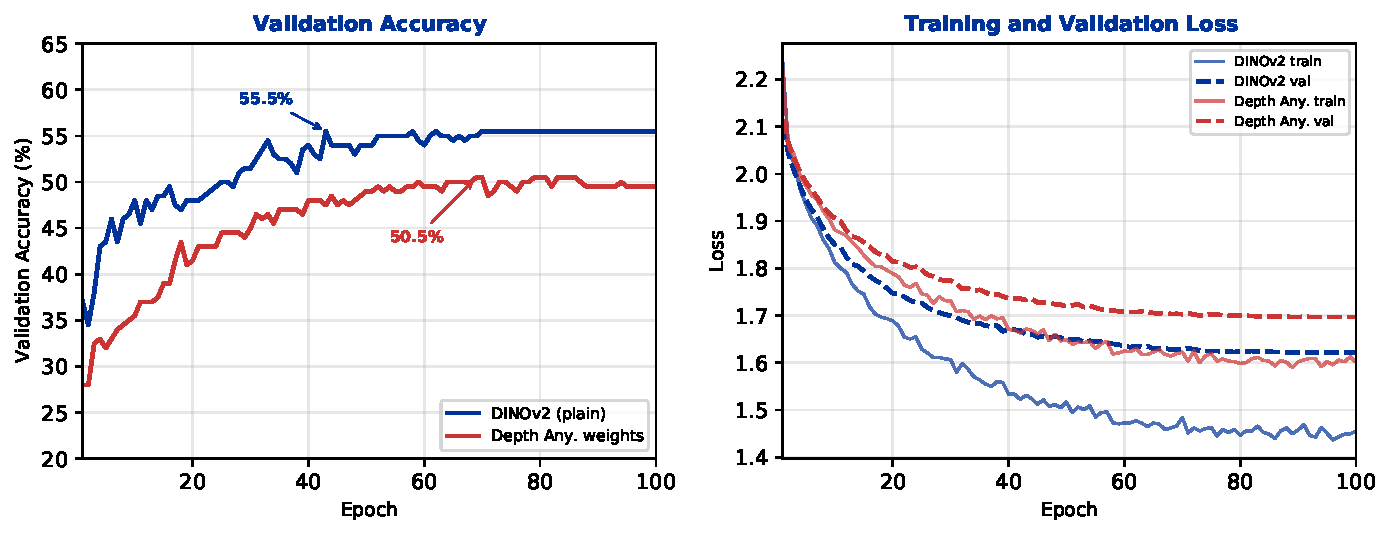
\includegraphics[width=\columnwidth]{figures/training_curves.pdf}
    \caption{Training dynamics. Left: validation accuracy. Right: loss curves.}
    \label{fig:training_curves}
\end{figure}

The model converges smoothly, reaching 55.5\% by approximately epoch 43 and maintaining this level through epoch 100.
The validation loss stabilizes early, confirming that the linear probe reaches its representational capacity limit for the frozen features.

\subsection{Comparison with the CLIP-Based Approach}

Prior to adopting the DINOv2 linear probing paradigm, we conducted experiments using CLIP ViT-B/32~\cite{clip} with an MLP adapter trained via NT-Xent contrastive loss.
This approach maps CLIP's 512-dimensional vision features to an aligned embedding space through cross-modal contrastive learning between RGB and depth representations.
Despite extensive hyperparameter tuning (learning rate, temperature, adapter depth, dropout), the best CLIP-based configuration achieved only 25.3\% on the 13-class validation set.

The fundamental limitation of the CLIP-based approach is that CLIP's vision encoder, pre-trained for image-text alignment, produces features that are not well-suited for depth-only inputs.
DINOv2's self-supervised features, in contrast, capture rich spatial and structural information that transfers naturally to depth maps.

\begin{table}[htb]
    \centering
    \caption{Comparison between CLIP-based and DINOv2-based approaches.}
    \label{tab:comparison}
    \footnotesize
    \begin{tabular}{lcc}
        \toprule
        \textbf{Dimension} & \textbf{CLIP + Adapter} & \textbf{Ours (DINOv2)} \\
        \midrule
        Backbone & CLIP ViT-B/32 & DINOv2-Base \\
        Training objective & Contrastive (NT-Xent) & Cross-entropy \\
        Trainable params & 528K & 10K \\
        Input resolution & 224$\times$224 & 518$\times$518 \\
        NYU13 accuracy & 25.3\% & \textbf{55.5\%} \\
        \bottomrule
    \end{tabular}
\end{table}

% ════════════════════════════════════════════
% V. DISCUSSION
% ════════════════════════════════════════════
\section{Discussion}

\subsection{Why Does DINOv2 Work on Depth Maps?}

DINOv2 has never ``seen'' a depth map during its pre-training---it is trained exclusively on RGB images.
Yet its features achieve competitive results on depth-only scene classification.
We attribute this to the nature of DINOv2's self-supervised learning objective.

DINOv2 is trained through self-distillation with masked image modeling and view consistency constraints.
This forces the model to learn features that capture scene-level semantics: object shapes, spatial layouts, and functional affordances of environments.
These semantic features are largely invariant to the input modality---whether represented as RGB values or depth values, a ``bedroom'' has a characteristic spatial structure that DINOv2's features can recognize.

In contrast, depth estimation pre-training (as in Depth Anything V2) optimizes for pixel-wise geometric accuracy, producing features that emphasize local depth gradients at the expense of global semantic abstraction.
While these geometric features are optimal for per-pixel regression, they are less suitable for scene-level classification.

\subsection{Efficiency Advantage}

A notable aspect of our approach is its parameter efficiency.
With only 10K trainable parameters (a single linear layer), we match the performance of methods that require full backbone fine-tuning with 25M--60M parameters.
This makes our approach highly practical for resource-constrained settings and rapid prototyping on new depth datasets.

\subsection{Limitations}

This study has several limitations.
First, the dataset (1,449 images) is relatively small, and our conclusions may not generalize to larger depth datasets such as SUN RGB-D.
Second, we evaluate only frozen backbone features; fine-tuning the DINOv2 backbone could potentially yield higher accuracy.
Third, the linear probing protocol, while clean for evaluation, may underutilize the full representational capacity of DINOv2 features.

% ════════════════════════════════════════════
% VI. CONCLUSION
% ════════════════════════════════════════════
\section{Conclusion}

We have demonstrated that DINOv2, a self-supervised vision transformer pre-trained exclusively on RGB images, serves as an effective feature extractor for depth map scene classification.
Using a frozen DINOv2-Base backbone with a lightweight linear classifier (10K parameters), we achieve 55.5\% Top-1 accuracy on the NYU Depth V2 13-class benchmark---competitive with fully fine-tuned depth-specific methods.

Our key findings are:

\begin{enumerate}
    \item Self-supervised RGB-pretrained features (DINOv2) effectively generalize to depth-only inputs for scene-level classification.
    \item Data augmentation contributes a 20.5 percentage point improvement, far exceeding the impact of architectural choices.
    \item With only 10K trainable parameters, our approach matches the performance of methods requiring millions of parameters and full backbone fine-tuning.
\end{enumerate}

These results establish DINOv2 as a strong baseline for depth map scene classification and highlight the potential of self-supervised RGB features for non-RGB sensor modalities.
Future work should explore fine-tuning regimes, larger depth datasets, and extension to other sensor types such as thermal infrared.

% ════════════════════════════════════════════
% REFERENCES
% ════════════════════════════════════════════
\begin{thebibliography}{00}

\bibitem{dinov2}
M. Oquab, T. Darcet, T. Moutakanni, \textit{et al.},
``DINOv2: Learning Robust Visual Features without Supervision,''
\textit{Transactions on Machine Learning Research}, 2024.

\bibitem{nyu_depth}
N. Silberman, D. Hoiem, P. Kohli, and R. Fergus,
``Indoor Segmentation and Support Inference from RGBD Images,''
in \textit{Proc. European Conference on Computer Vision (ECCV)}, 2012.

\bibitem{gupta2014indoor}
S. Gupta, R. Girshick, P. Arbel{\'a}ez, and J. Malik,
``Learning Rich Features from RGB-D Images for Object Detection and Segmentation,''
in \textit{Proc. European Conference on Computer Vision (ECCV)}, 2014.

\bibitem{robotics_depth}
K. He, G. Gkioxari, P. Doll{\'a}r, and R. Girshick,
``Mask R-CNN,''
in \textit{Proc. IEEE Int. Conf. Computer Vision (ICCV)}, 2017.

\bibitem{wang2016depth}
A. Wang, J. Lu, J. Cai, \textit{et al.},
``Unsupervised Joint Feature Learning for Zero-shot Scene Classification,''
arXiv:1609.00245, 2016.

\bibitem{rednet}
J. Jiang, L. Zheng, F. Luo, and Z. Zhang,
``RedNet: Residual Encoder-Decoder Network for Indoor RGB-D Semantic Segmentation,''
arXiv:1806.01054, 2018.

\bibitem{clip}
A. Radford, J. W. Kim, C. Hallacy, \textit{et al.},
``Learning Transferable Visual Models From Natural Language Supervision,''
in \textit{Proc. Int. Conf. Machine Learning (ICML)}, 2021.

\bibitem{alain2016understanding}
G. Alain and Y. Bengio,
``Understanding intermediate layers using linear classifier probes,''
in \textit{ICLR Workshop}, 2017.

\bibitem{project_summary}
Mar-Ding,
``Depth Scene Classification: Project Summary,''
Technical report, 2026.
\url{https://github.com/Mar-Ding/depth-scene-classification}

\end{thebibliography}

\end{document}
